\section{Vytvorenie druhého ramena}

V rámci riešenia tímového projektu sme dostali za úlohu nielen teoreticky opísať kinematiku a vytvoriť softvérové riadenie, ale tiež si prakticky vyskúšať proces mechanického návrhu. Naším cieľom bolo navrhnúť vlastný modul, respektíve vytvoriť a odladiť aspoň jeden funkčný kĺb manipulátora. Chceli sme sa tak bližšie oboznámiť s princípmi CAD modelovania. 

Vzhľadom na časovú a technickú náročnosť navrhovania celého kinematického reťazca úplne od základov, sme sa rozhodli pre efektívnejší prístup. Vybrali sme si voľne dostupný a komunitou overený open-source model robotického ramena, ktorý nám poslúžil ako robustný základ. Našou pridanou hodnotou a hlavnou konštruktérskou úlohou bolo tento model modifikovať a rozšíriť ho o vlastný, na mieru modelovaný kĺb. Tento proces nám poskytol veľmi cenné skúsenosti z reálneho sveta, najmä pri riešení problémov so súosovosťou, mechanickými toleranciami plastov a celkovou konštrukčnou tuhosťou.

\subsection{Východiskový model robotického ramena}
Na nasledujúcich obrázkoch (Obrázok \ref{fig:obr1}, Obrázok \ref{fig:obr2}) je možné vidieť pôvodný návrh robotického ramena z: \href{https://makerworld.com/en/models/1134925-robotic-arm-with-servo-arduino?from=search#profileId-1135927}{\textit{Robotic Arm with Servo \& Arduino - Free 3D Print Model - MakerWorld}}.

\begin{figure}[htbp]
    \centering
    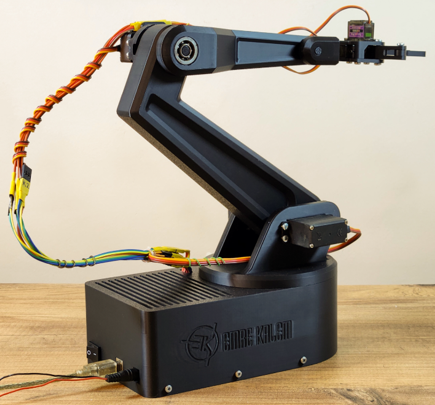
\includegraphics[width=0.7\textwidth]{img/obr_1.png}
    \caption{Konštrukcia celého robotického ramena}
    \label{fig:obr1}
\end{figure}

\begin{figure}[htbp]
    \centering
    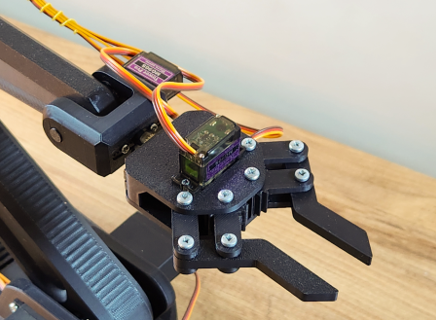
\includegraphics[width=0.7\textwidth]{img/obr_2.png}
    \caption{Konštrukcia Grippera}
    \label{fig:obr2}
\end{figure}

\subsection{Úprava robotického ramena}
Pre náš návrh robota sme sa robotické rameno rozhodli rozšíriť o jeden kĺb v y-osi, čím došlo k zvýšeniu jeho stupňov voľnosti z 5 DOF na 6 DOF. Obrázky \ref{fig:obr3} a \ref{fig:obr4} zobrazujú CAD návrhy rozšírených súčiastok určených na prerobenie koncových častí s efektorom pre vyššie uvedené robotické rameno.

\begin{figure}[htbp]
    \centering
    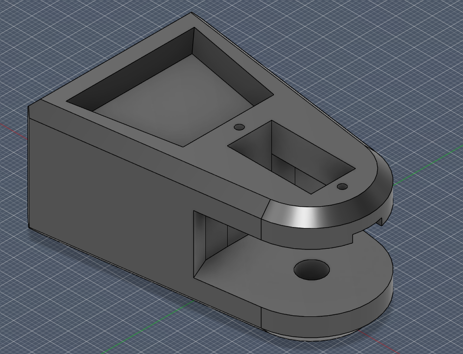
\includegraphics[width=0.7\textwidth]{img/obr_3.png}
    \caption{Kĺb na držanie mikroservo motorov pre osi "z" a "y"}
    \label{fig:obr3}
\end{figure}

\begin{figure}[htbp]
    \centering
    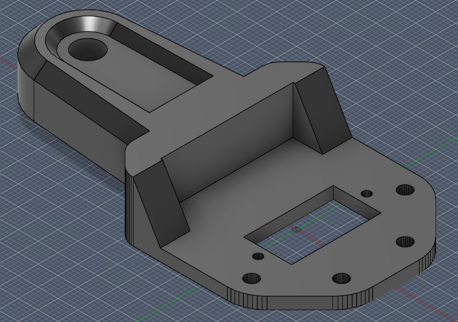
\includegraphics[width=0.7\textwidth]{img/obr_4.png}
    \caption{Uchopovacia súčiastka pre mikroservo patriace Gripperu}
    \label{fig:obr4}
\end{figure}

\subsection{Finálna konštrukcia robota a jej problémy}
Počas konštrukcie robota nastalo niekoľko chýb obmedzujúcich správnu funkčnosť robota, spôsobených návrhom jednotlivých segmentov, kvalitou materiálu a kvalitou tlače robota. Väčšina problémov bola odstránená, prípadne čiastočne opravená tak, aby robot dokázal fungovať.

\begin{figure}[htbp]
    \centering
    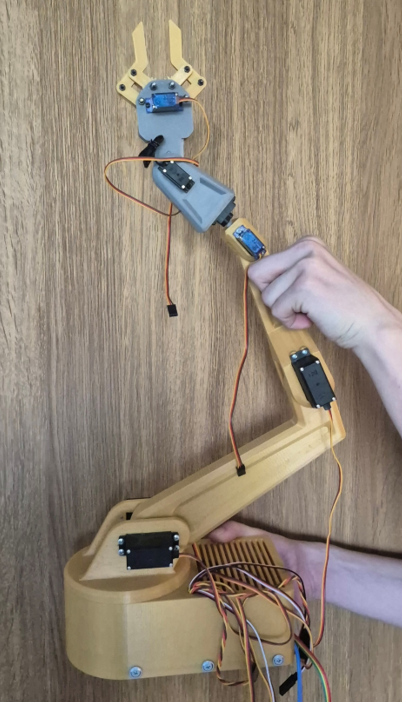
\includegraphics[width=0.6\textwidth]{img/obr_5.png}
    \caption{Kompletná konštrukcia modifikovaného ramena}
    \label{fig:obr5}
\end{figure}

Na Obrázku \ref{fig:obr5} je možné vidieť finálnu konštrukciu robotického ramena. Jednotlivé servo motory dočasne neboli zapojené.

Na Obrázku \ref{fig:obr6} sú červeným ohraničením zvýraznené spomínané konštrukčné komplikácie. Nastali konkrétne dva unikátne problémy. Prvý bol spôsobený zvýšenou záťažou na osku mikroserva, kedy plastový socket nedokázal zvyšok konštrukcie so servom udržať (bol pripevnený k servu pomocou skrutky). Tento defekt inak neovplyvnil schopnosť mikroserva. Druhý problém predstavovali široké drážky medzi kĺbmi, ktoré spôsobovali nedoliehanie mikroservo motorov do ich socketov. Tento problém bol vyriešený pomocou kovových podložiek a stabilizačných kolíkov.

\begin{figure}[htbp]
    \centering
    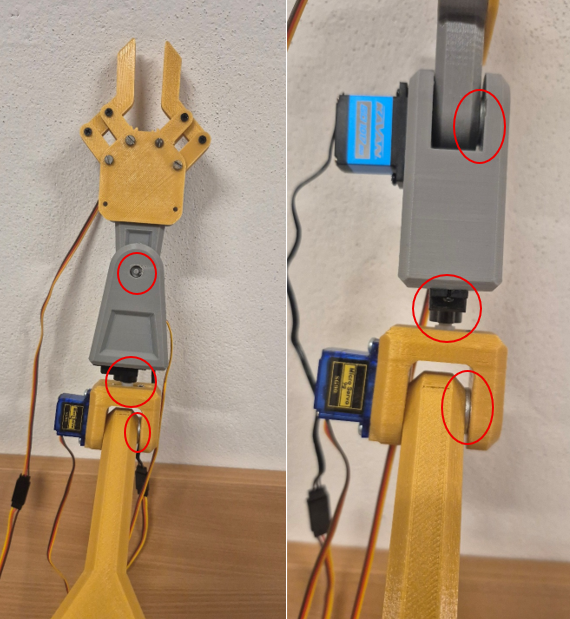
\includegraphics[width=0.8\textwidth]{img/obr_6.png}
    \caption{Konštrukčné problémy ramena}
    \label{fig:obr6}
\end{figure}
